% ПРОЧИТАЙ МЕНЯ
% ПРОЧИТАЙ МЕНЯ
% ПРОЧИТАЙ МЕНЯ
% 
% В этом файле вы описываете задачи из контеста
% Условия можно вставить в виде фотографий
% В идеях нужно написать хотя бы два-три предложения о задаче
% Если задача довольно трудная, описание идеи должно быть подробным
% Комментарии в исходном коде приветствуются
% Положение тоже можно фотографией
%
% ПРОЧИТАЙ МЕНЯ
% ПРОЧИТАЙ МЕНЯ
% ПРОЧИТАЙ МЕНЯ

\subsection*{Codeforces Round \#768 (Div. 2)}
\begin{center}
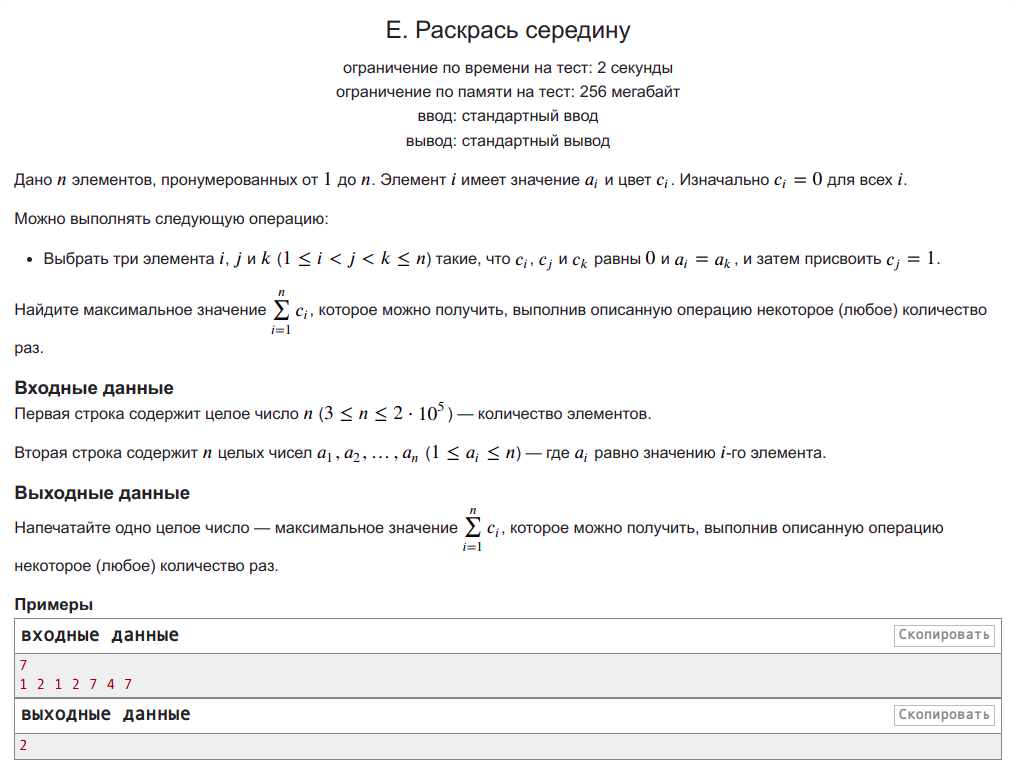
\includegraphics[scale=0.5]{statements/sample-cf.png}
\end{center}
\subsubsection*{Идея}
Тут вы описываете идею решения, оцениваете сложность...

{\bfseries \large Например}

Переборное решение работает $O(n!)$, это очень долго. Использую метод динамического программирования, $dp_i$ --- это минимальное количество белочек при условии чего-то там для $i$ веточек. Это позволяет решить задачу за $O(n ^ 2)$. Дерево отрезков с отложенными обновлениями позволяет улучшить асимптотику до $O(n \cdot \log{n})$, так как все операции с деревом соврешаются за $O(\log{n})$.

\subsubsection*{Исходный код}
\lstinputlisting{src/sample-cf-e.cpp}

\subsubsection*{Положение}
\begin{center}
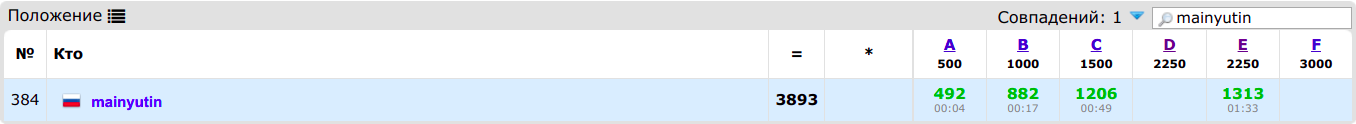
\includegraphics[scale=0.35]{standings/sample-cf.png}\newline\noindent
\end{center}
\pagebreak
